%%%%%%%%%%%%%%%%%%%%%%%%%%%%%%%%%%%%%%%%%%%%%%%%%%%%%%%%%%%%%%%%%%%%%%
% Lớp 11 | Dãy số. Cấp số cộng. Cấp số nhân | Cấp số cộng
% Dạng 1D2?2-3: Số hạng tổng quát của cấp số cộng
% Số câu: 56  (sinh tự động bởi tach_cau.py; từ nay thầy sửa trực tiếp file này)
%%%%%%%%%%%%%%%%%%%%%%%%%%%%%%%%%%%%%%%%%%%%%%%%%%%%%%%%%%%%%%%%%%%%%%

%%%%%%%%%%%%%%%% TRẮC NGHIỆM 4 PHƯƠNG ÁN %%%%%%%%%%%%%%%%

% nguồn: Ok_Toan11_TracNghiem_Lan2
\begin{ex}%[1D2N2-3]%[ma:583e8b56]
	Trong các dãy số có công thức tổng quát sau, dãy số $(u_n)$ nào là  cấp số cộng?
	\choice 
		{$u_n={{2\,021}^n}$} 
		{\True $u_n=2n+2\,021$} 
		 {$u_n=\dfrac{2}{n+2\,021}$}
		 {$u_n={n^2}-2$}
	\loigiai{ 
		Với $u_n=2n+2\,021$ thì ${u_{n+1}}=2(n+1)+2\,021=u_n+2$, như vậy dãy số này là một cấp số cộng. 
	 }
\end{ex}

% nguồn: Ok_Toan11_TracNghiem_Lan2
\begin{ex}%[1D2N2-3]%[ma:2d7557ca]
	Trong các dãy  số sau, dãy số nào là cấp số cộng?
	 \choice
		{$4;\, 8;\, 16;\, 32$} 
		{\True $4;\, 6;\, 8;\, 10$} 
		 {$-1;\, 1;\,-1;\, 1$}
		{$3;\, 5;\, 7;\, 10$} 
	\loigiai{ 
		Ta có $6=4+2;\, 8=6+2;\, 10=8+2$.\\ 
		Nên dãy số $4;\, 6;\, 8;\, 10$ là một cấp  số cộng.
	} 
\end{ex}

% nguồn: Ok_Toan11_TracNghiem_Lan2
\begin{ex}%[1D2N2-3]%[ma:7ffa6397]
	Cho cấp số cộng $(u_n)$ có  các số hạng đầu lần lượt là $5; \ 9; \ 13; \ 17; \ \ldots$. Số hạng tổng quát $u_n$ của cấp số cộng là
	 \choice
		 {$u_n=5n+1$}
		{$u_n=5n-1$} 
		{\True $u_n=4n+1$} 
		{$u_n=4n-1$} 
	\loigiai{ 
		Các số $5; \, 9; \, 13; \, 17; \  \ldots$ lập thành cấp số cộng với
		\[ 
		u_1=5,\, d=u_2-u_1=9-5=4. 
		\] 
		Sử dụng công thức tổng quát ta được 
		 \[
		 u_n=u_1+(n-1)d=5+(n-1)4=5+4n-4=4n+1.
		\] 
		Vậy số hạng tổng quát là ${u_n=4n+1}$. 
	} 
\end{ex}

% nguồn: Ok_Toan11_TracNghiem_Lan2
\begin{ex}%[1D2N2-3]%[ma:779713d9]
	Tìm công thức số hạng tổng quát của cấp số cộng  $(u_n)$ thỏa mãn:
	$\heva{&u_2-u_3+u_5=7\\ &u_1+u_4=12.}$ 
	\choice 
		 {$u_n=2n+3$}
		 {\True $u_n=2n-1$}
		{$u_n=2n+1$} 
		 {$u_n=2n-3$}
	\loigiai{ 
		 Giả sử dãy cấp số cộng $(u_n)$ có công sai là $d$.\\
		Khi đó, hệ phương  trình
		 $\heva{&u_2-u_3+u_5=7\\&u_1+u_4=12}$
		 trở thành\\
		\[\heva{ &(u_1+d)-(u_1+2d)+(u_1+4d)=7\\&  u_1+(u_1+3d)=12}\Leftrightarrow \heva{ &u_1+3d=7\\ &2u_1+5d=12 } \Leftrightarrow \heva{& u_1=1\\& d=2.} \]
		Số hạng tổng quát  của cấp số cộng $(u_n)$ là $u_n=u_1+(n-1)d=1+(n-1)\cdot2=2n-1$.\\
		Vậy  $u_n=2n-1$.
	} 
\end{ex}

% nguồn: Ok_Toan11_TracNghiem_Lan2
\begin{ex}%[1D2N2-3]%[ma:1ac45922]
	 Trong các dãy số $(u_n)$ sau đây, dãy số nào là cấp số cộng?
	 \choice
		{$\left\{\begin{aligned}
		&u_1=3\\ 
		 &u_{n+1}=2u_n+1
\end{aligned}\right.$}
{\True $\left\{\begin{aligned}
 &u_1=-1\\
 &u_{n+1}-u_n=2
\end{aligned}\right.$}
{$\left\{\begin{aligned}
 &u_1=1\\
 &u_{n+1}=u_n^3-1
\end{aligned}\right.$}
{$\left\{\begin{aligned}
 &u_1=1\\
&u_{n+1}=u_n+n 
\end{aligned}\right.$}
\loigiai{ 
	 Xét dãy số $\heva{&u_1=-1\\&u_{n+1}-u_n=2.}$\\
	Vì $u_{n+1}-u_n=2$ với mọi $n \in \mathbb{N}^*$ nên $(u_n)$ là cấp số  cộng có $u_1=-1; d=2$.
} 
\end{ex}

% nguồn: Ok_Toan11_TracNghiem_Lan2
\begin{ex}%[1D2N2-3]%[ma:7e853a25]
	Trong các dãy số $(u_n)$ sau đây, dãy số nào là cấp  số cộng?
	\choice 
		 {$u_n=3{n^2}+2\,017$}
		 {\True $u_n=3n+2\,018$}
		 {$u_n={3^n}$}
		{$u_n=(-3)^{n+1}$} 
	 \loigiai{
		Ta có $u_{n+1}-u_n=3(n+1)+2\,018-(3 n+2\,018)=3\Leftrightarrow u_{n+1}=u_n+3$.  \\
		 Vậy dãy số trên là cấp số cộng có công sai $d=3$.
	 }
\end{ex}

% nguồn: Ok_Toan11_TracNghiem_Lan2
\begin{ex}%[1D2N2-3]%[ma:48f59af6]
	Cho cấp  số cộng có $u_1=-2$ và $d=4$. Chọn khẳng định đúng trong các khẳng định sau?
	\choice 
		{$u_4=8$} 
		 {$u_5=15$}
		{$u_2=3$} 
		{\True  $u_3=6$}
	 \loigiai{
		Ta có $u_1=-2$ và $d=4$. 
		Suy ra  $$u_2=u_1+d=-2+4=2$$
		$$u_3=u_1+2d=-2+2\cdot4=6$$ 
		$$u_5=u_1+4d=-2+4\cdot4=14$$ 
		$$u_4=u_1+3d=-2+3\cdot4=10.$$ 
	 }
\end{ex}

% nguồn: Ok_Toan11_TracNghiem_Lan2
\begin{ex}%[1D2N2-3]%[ma:2d3a8d1b]
	Dãy số $(u_n)$  nào sau đây là cấp số cộng?
	 \choice
		{$(u_n):  u_n=\dfrac{1}{n}$}
		{\True $(u_n): u_n={u_{n-1}}-2, \forall n\ge  2$}
		{$(u_n):  u_n={2^n}-1$}
		 {$(u_n): u_n=2{u_{n-1}}, \forall n\ge 2$}
	 \loigiai{
		Xét dãy số $(u_n): u_n={u_{n-1}}-2,  \forall n\ge 2$.\\
		Ta  có $u_n-{u_{n-1}}=-2, \forall n\ge 2$.\\
		Vậy  dãy số đã cho là cấp số cộng với công sai $d=-2$.
	 }
\end{ex}

% nguồn: Ok_Toan11_TracNghiem_Lan2
\begin{ex}%[1D2N2-3]%[ma:7f742a6d]
	Trong các dãy số $(u_n)$ sau, dãy nào là  cấp số cộng?
	 \choice
		 {$u_n={3^{n+1}}$}
		{$u_n=\dfrac{2}{n+1}$} 
		{$u_n=\sqrt{{n^2}+1}$} 
		{\True  $u_n=\dfrac{5n-2}{3}$}
	 \loigiai{
		Ta có dãy $u_n$  là cấp số cộng khi $u_{n+1}-u_n=d, \forall \text{ n }\in \mathbb{N}^{*}$ với $d$ là hằng số. \\
		Xét hiệu  $u_{n+1}-u_n=\dfrac{5\left(n+1\right)-2}{3}-\dfrac{5 n-2}{3}=\dfrac{5}{3}\text{, }\forall \text{ n }\in \mathbb{N}^{*}$. \\
		Vậy dãy $u_n=\dfrac{5n-2}{3}$ là cấp số  cộng.
	 }
\end{ex}

% nguồn: Ok_Toan11_TracNghiem_Lan2
\begin{ex}%[1D2N2-3]%[ma:02d42bde]
	Trong các dãy số sau, dãy nào  là một cấp số cộng?
	\choice 
		 {$1;-3;-6;-9;-12$}
		 {\True $1;-3;-7;-11;-15$}
		{$1;-3;-5;-7;-9$} 
		{$1;-2;-4;-6;-8$} 
	 \loigiai{
		Ta có  dãy số $1;-3;-7;-11;-15$ là một cấp số cộng có công sai $d=-4$.
	} 
\end{ex}

% nguồn: Ok_Toan11_TracNghiem_Lan2
\begin{ex}%[1D2N2-3]%[ma:c5c4849e]
	Trong các dãy  số $(u_n)$ sau đây, dãy số nào là cấp số cộng?
	 \choice
		 {$u_n=3^n$}
		 {$u_n=(-3)^{n+1}$}
		{\True  $u_n=3n+1$}
		{$u_n=2^{n+1}$} 
	 \loigiai{
		Xét dãy số $u_n=3n+1$.  Ta có\\
		 $$
		u_{n+1}-u_n=[3(n+1)+1]-(3n+1)=3 \Rightarrow \text{ không  đổi }\Rightarrow u_n=3n+1 \text{ là cấp số cộng. }
		 $$
	} 
\end{ex}

% nguồn: Ok_Toan11_TracNghiem_Lan2
\begin{ex}%[1D2N2-3]%[ma:9383db0a]
	Cho cấp số  cộng $(u_n)$ có $u_1=-3$ và $d=\dfrac{1}{2}$. Khẳng định nào sau đây đúng?
	 \choice
		 {$u_n=-3+\dfrac{1}{2}(n+1)$}
		 {$u_n=-3+\dfrac{1}{2}n-1$}
		{\True $u_n=-3+\dfrac{1}{2}(n-1)$} 
		{$u_n=-3+\dfrac{1}{4}(n-1)$} 
	\loigiai{ 
		Ta áp dụng công thức tổng quát của  cấp số cộng
		 \[
		u_n=u_1+(n-1)d. 
		 \]
		Với $u_1=-3$, $d=\dfrac{1}{2}$,ta  có
		 \[
		u_n=-3+\dfrac{1}{2}(n-1). 
		 \]
		Vậy đáp án đúng là ${u_n=-3+\dfrac{1}{2}(n-1)}$. 
	} 
\end{ex}

% nguồn: Ok_Toan11_TracNghiem_Lan2
\begin{ex}%[1D2N2-3]%[ma:a729fdce]
	Trong các dãy số $(u_n)$ sau đây, dãy số nào là một cấp số cộng? 
	 \choice
		 {$u_n=n^2+1,\, n \ge 1$}
		 {$u_n=2^n,\, n \ge 1$}
		{$u_n=\sqrt{n+1},\, n \ge 1$} 
		 {\True $u_n=2n-3,\, n \ge 1$}
	\loigiai{ 
		Theo định  nghĩa, dãy số $(u_n)$ là cấp số cộng khi tồn tại hằng số $d$ sao cho $u_{n+1}-u_n=d, \forall n \ge 1$. \\
		Xét dãy $u_n=2n-3, \,  n \ge 1$, ta có
		\[ 
		\begin{aligned}
			u_n  &=2n-3; \\
			u_{n+1}  &=2(n+1)-3=2n-1; \\
			\Rightarrow u_{n+1}-u_n &=(2n-1)-(2n-3)=2. 
		\end{aligned}
		 \]
		Vì hiệu $u_{n+1}-u_n=2$  là không đổi nên đây là một cấp số cộng với công sai $d=2$.
	 }
\end{ex}

% nguồn: Ok_TracNghiemLop11_Lan1
\begin{ex}%[1D2N2-3]%[ma:7dd6cb70]
	Cho cấp số  cộng $(u_n)$ với số hạng đầu $u_1=-3$ và công sai $d=\dfrac{1}{2}$. Công thức số hạng tổng quát của $(u_n)$ là
	 \choice
		{$u_n=-3+\dfrac{1}{2}n-1$} 
		 {\True $u_n=-\dfrac{7}{2}+\dfrac{1}{2}n$}
		{$u_n=-\dfrac{5}{2}+\dfrac{1}{2}n$} 
		{$u_n=-\dfrac{11}{4}+\dfrac{1}{4}n$} 
	 \loigiai{
		Ta có  $u_n=u_1+(n-1)d=-3+\dfrac{1}{2}(n-1)=-\dfrac{7}{2}+\dfrac{1}{2}n$.
	 }
\end{ex}

% nguồn: Ok_TracNghiemLop11_Lan1
\begin{ex}%[1D2N2-3]%[ma:17a692ae]
	Cho cấp số cộng  $(u_n)$ biết số hạng đầu $u_1=5$ và công sai $d=4$. Số hạng tổng quát của cấp số cộng là
	 \choice
		{ $u_n=4n-1$} 
		{ $u_n=5n+1$} 
		{\True $u_n=4n+1$} 
		{ $u_n=5n-1$} 
	 \loigiai{
		Ta có công thức xác định số hạng tổng quát của cấp số cộng $u_n=u_1+(n-1)d$  nên $u_n=5+(n-1)\cdot 4=4n+1$
	 }
\end{ex}

% nguồn: Ok_TracNghiemLop11_Lan1
\begin{ex}%[1D2N2-3]%[ma:6a98af77]
	Cho cấp  số cộng $(u_n)$ có $u_1=3$ và $u_2=-1$.
	Khi  đó
	 \choice
		 {$u_3=4$}
		{$u_3=2$} 
		 {\True $u_3=-5$}
		 {$u_3=7$}
	 \loigiai{
		Ta có $u_2=u_1+d\Rightarrow d=u_2-u_1=-1-3=-4$.\\ 
	Suy ra  $u_3=u_1+2d=3-8=-5$.}
\end{ex}

% nguồn: Ok_TracNghiemLop11_Lan1
\begin{ex}%[1D2N2-3]%[ma:22b8db02]
	Cho cấp số cộng $(u_n)$  có số hạng thứ hai $u_2=5$ và số hạng thứ ba là $u_3=8$. Tìm số hạng đầu $u_1$ và công sai $d$ của cấp số cộng đó?
	\choice 
		{$u_1=1;d=3$} 
		 {\True $u_1=2;d=3$}
		 {$u_1=3;d=2$}
		{$u_1=2;d=-3$} 
	 \loigiai{
	Ta có $d=u_3-u_2=3$;  $u_1=u_2-d=2$.}
\end{ex}

% nguồn: Ok_Toan11_TracNghiem_Lan2
\begin{ex}%[1D2H2-3]%[ma:d8745bd6]
	Cho cấp  số cộng có số hạng thứ $3$ và số hạng thứ $7$ lần lượt là $6$ và $-2$. Tìm số hạng thứ $5$.
	 \choice
		 {\True $u_5=2$}
		{$u_5=-2$} 
		{$u_5=0$} 
		{$u_5=4$} 
	 \loigiai{
		Theo giả thiết ta có $\heva{& u_3=6\\& u_7=-2} \Leftrightarrow \heva{& u_1+2\cdot d=6\\& u_1+6\cdot d=-2} \Leftrightarrow \heva{&  d=-2\\& u_1=10.}$\\
		Vậy  $u_5=u_1+4\cdot d=10+4\cdot (-2)=10-8=2$.
	} 
\end{ex}

% nguồn: Ok_Toan11_TracNghiem_Lan2
\begin{ex}%[1D2H2-3]%[ma:02729610]
	Cho cấp số cộng $(u_n)$ có $\heva  {& u_1 - 2u_5 + u_6 = -15\\& u_3 + u_7 = 46}$. Số hạng đầu $u_1$ là
	\choice 
		 {$u_1 = -5$}
		{$u_1 =  5$}
		 {\True $u_1 = 3$}
		{$u_1 =  -3$}
	\loigiai{ 
		Ta có 
		\begin{align*}
			&\quad \heva{& u_1-2u_5+u_6=-15\\&  u_3+u_7=46}\\
			&\Leftrightarrow \heva{& u_1-2(u_1+4\cdot d)+(u_1+5\cdot d)=-15\\&  (u_1+2\cdot d)+(u_1+6\cdot d)=46}\\
			 &\Leftrightarrow \heva{& d=5\\& 2u_1+8\cdot d=46}\\
			 &\Rightarrow u_1=3.
		\end{align*}
	} 
\end{ex}

% nguồn: Ok_Toan11_TracNghiem_Lan2
\begin{ex}%[1D2H2-3]%[ma:5e0ede39]
	Một cấp số cộng có số hạng đầu $u_1 = 2\,018$ công sai $d = -5$. Hỏi bắt  đầu từ số hạng nào của cấp số cộng đó thì nó nhận giá trị âm.
	 \choice
		 {$u_{406}$}
		{$u_{403}$} 
		{\True $u_{405}$} 
		{$u_{404}$} 
	\loigiai{ 
		 Ta có $u_n = u_1 + (n-1)\cdot d = 2\,018-5\cdot (n-1)$.\\
		Có $u_n < 0 \Leftrightarrow 2\,018-5\cdot (n-1) < 0 \Leftrightarrow 5n > 2\,023 \Leftrightarrow n > \dfrac{2\,023}{5}$, $n  \in \mathbb{Z} \Rightarrow n \ge 405$.\\
		Vậy từ $u_{405}$ thì  số hạng của cấp số cộng đó nhận giá trị âm.
	 }
\end{ex}

% nguồn: Ok_Toan11_TracNghiem_Lan2
\begin{ex}%[1D2H2-3]%[ma:547cccc1]
	Cho dãy  số $(u_n)$ xác định bởi $\heva{& u_1 = 2\\& u_{n+1} = u_n + 5, n \in \mathbb{N}^*}$. Tính $u_{10}$.
	\choice 
		{$57$} 
		{$62$} 
		 {\True $47$}
		 {$52$}
	\loigiai{ 
		Từ $\heva{& u_1 = 2\\& u_{n+1} = u_n + 5,  n \in \mathbb{N}^*.}$\\
		 Ta có $u_{n+1} - u_n = 5$ nên dãy $(u_n)$ là một cấp số cộng với công sai $d = 5$.\\
		Nên $u_{10} = u_1 + 9\cdot d = 2 + 9 \cdot  5 = 47$.
	 }
\end{ex}

% nguồn: Ok_Toan11_TracNghiem_Lan2
\begin{ex}%[1D2H2-3]%[ma:c61a82dd]
	Cho cấp số cộng $(u_n)$ có $u_1=123$ và $u_3-u_{15}=84$. Số $11$ là số hạng thứ  bao nhiêu của cấp số cộng đã cho.
	 \choice
		 {\True $17$}
		{$16$} 
		{$18$} 
		 {$19$}
	 \loigiai{
		Ta có $u_3-u_{15}=84 \Leftrightarrow u_1+2\cdot  d-(u_1+14\cdot d)=84 \Leftrightarrow d=-7$.\\
		Số hạng tổng quát  $u_n=-7n+130$.\\
		 Ta có $u_n=11 \Leftrightarrow -7n+130=11 \Leftrightarrow 7n=119 \Leftrightarrow n=17$.
	 }
\end{ex}

% nguồn: Ok_Toan11_TracNghiem_Lan2
\begin{ex}%[1D2H2-3]%[ma:634fff11]
	Cho cấp số cộng $(u_n)$ có số hạng đầu là $u_2 = 1$; $u_5  = 19$. Số $103$ là số hạng thứ mấy trong cấp số cộng đã cho.
	\choice 
		{\True $19$} 
		 {$18$}
		{$20$} 
		 {$17$}
	\loigiai{ 
		Ta có $\heva{& u_2 = 1\\& u_5 = 19} \Leftrightarrow \heva{& u_1 + d = 1\\& u_1 + 4\cdot d = 19}  \Leftrightarrow \heva{& u_1 = -5\\& d = 6.}$\\
		Lại có $u_n  = u_1 + (n-1)\cdot d \Leftrightarrow 103 = -5 + (n-1)\cdot 6 \Leftrightarrow n = 19$.\\
		Vậy số $103$ là số  hạng thứ $19$ trong cấp số cộng đã cho.
	 }
\end{ex}

% nguồn: Ok_Toan11_TracNghiem_Lan2
\begin{ex}%[1D2H2-3]%[ma:eb285e3c]
	Cho cấp số cộng $(u_n)$  có $u_1 = 5$ và công sai $d = -3$. Biết rằng $-289$ là một số hạng của cấp số cộng trên. Hỏi đó là số hạng thứ bao nhiêu.
	\choice 
		 {$98$}
		{\True $99$} 
		{$101$} 
		 {$100$}
	 \loigiai{
		 Số hạng tổng quát của cấp số cộng có $u_1 = 5$ và công sai $d = -3$ là $u_n = 5-3\cdot (n-1)$, $\forall n \in \mathbb{N}^*$.\\
		Ta có $-289 = 5-3\cdot (n-1) \Leftrightarrow  -294 = -3\cdot (n-1) \Leftrightarrow 98 = n-1 \Leftrightarrow n = 99$.\\
		Vậy $-289$ là số hạng thứ $99$ của cấp số cộng  trên.
	} 
\end{ex}

% nguồn: Ok_Toan11_TracNghiem_Lan2
\begin{ex}%[1D2H2-3]%[ma:c35bdf43]
	Cho cấp số cộng $(u_n)$ biết $u_1=3$;  $u_8=24$ thì $u_{11}$ bằng
	 \choice
		 {$30$}
		{\True  $33$}
		 {$32$}
		 {$28$}
	 \loigiai{
		Ta có $u_8=u_1+7\cdot d \Leftrightarrow  d=\dfrac{u_8-u_1}{7}=\dfrac{24-3}{7}=3$; $u_{11}=u_1+10\cdot d=33$.
	 }
\end{ex}

% nguồn: Ok_Toan11_TracNghiem_Lan2
\begin{ex}%[1D2H2-3]%[ma:b8b91e46]
	Cho cấp số cộng $(u_n)$ thỏa mãn $\heva{& u_5 + 3u_3 - u_2 = -21\\& 3u_7 -  2u_4 = -34}$. Tính số hạng thứ $100$ của cấp số.
	 \choice
		{$u_{100} = -243$} 
		{\True $u_{100} = -295$} 
		{$u_{100} = -231$} 
		 {$u_{100} = -294$}
	 \loigiai{
		Ta  có
		\begin{align*}
			&\quad \heva{& u_5  + 3u_3 - u_2 = -21\\& 3u_7 - 2u_4 = -34}\\
			&\Leftrightarrow \heva{& (u_1 + 4\cdot d) + 3(u_1 + 2\cdot d) - (u_1 + d) = -21\\& 3(u_1 + 6\cdot d) - 2(u_1 + 3\cdot d)  = -34}\\
			&\Leftrightarrow \heva{& u_1 + 3\cdot d = -7\\ &u_1 + 12\cdot d = -34}\\ &\Leftrightarrow \heva{& u_1 =  2\\& d = -3.}
		\end{align*}
		Số  hạng thứ $100$ là $u_{100} = u_1 + 99\cdot d = 2 + 99\cdot (-3) = -295$.
	} 
\end{ex}

% nguồn: Ok_Toan11_TracNghiem_Lan2
\begin{ex}%[1D2H2-3]%[ma:182acd16]
	Cho một cấp số cộng $(u_n)$ có $u_1=5$ và tổng của $50$ số hạng đầu bằng $5\,150$. Tìm  công thức của số hạng tổng quát $u_n$.
	\choice 
		{\True $u_n=1+4n$} 
		 {$u_n=5n$}
		 {$u_n=3+2n$}
		 {$u_n=2+3n$}
	\loigiai{Ta  có $S_{50}=\dfrac {50}{2}(2u_1+49d)=5\,150 \Rightarrow d=4$.\\
		Số hạng tổng quát của cấp số cộng bằng  $u_n=u_1+(n-1)d=1+4n$.
	} 
\end{ex}

% nguồn: Ok_Toan11_TracNghiem_Lan2
\begin{ex}%[1D2H2-3]%[ma:a72acf02]
	Cho cấp số  cộng $(u_n)$ có $u_1=3$ và công sai $d=7$. Hỏi kể từ số hạng thứ mấy trở đi thì các số hạng của $(u_n)$ đều lớn hơn $2\,018$.
	 \choice
		{$287$} 
		{\True  $289$}
		{$288$} 
		 {$286$}
	\loigiai{ 
		Ta có $u_n = u_1  + (n-1)\cdot d = 3 + 7\cdot (n-1) = 7n-4$.\\
		 $u_n > 2\,018 \Leftrightarrow 7n-4 > 2\,018 \Leftrightarrow n > \dfrac{2\,022}{7}$.\\
		 Vậy $n=289$.
	 }
\end{ex}

% nguồn: Ok_Toan11_TracNghiem_Lan2
\begin{ex}%[1D2H2-3]%[ma:3cc90a53]
	Cho cấp số cộng $(u_n)$,  biết $u_1 = -5$; $d = 2$. Số $81$ là số hạng thứ bao nhiêu?
	 \choice
		{$100$} 
		{$50$} 
		 {$75$}
		{\True  $44$}
	 \loigiai{
		Ta có $u_n = u_1 + (n-1)\cdot  d \Leftrightarrow 81 = -5 + (n-1)\cdot 2 \Leftrightarrow n = 44$.\\
		 Vậy $81$ là số hạng thứ $44$.
	} 
\end{ex}

% nguồn: Ok_Toan11_TracNghiem_Lan2
\begin{ex}%[1D2H2-3]%[ma:0198b805]
	Cho cấp số cộng $u_n$ có các số hạng đầu lần lượt là $5;9;13;17;\ldots$. Tìm số hạng tổng quát $u_n$ của cấp số  cộng?
	\choice 
		{\True  $u_n=4n+1$}
		 {$u_n=5n-1$}
		 {$u_n=5n+1$}
		{$u_n=4n-1$} 
	\loigiai{Cấp số cộng $u_n$ có các  số hạng đầu lần lượt là $5;9;13;17;\ldots$ có $u_1=5$ và $d=4$. \\
		Vậy số hạng tổng quát của $(u_n)$  là $u_n=u_1+(n-1)d=5+4(n-1)=5+4n-4=4n+1$.
	} 
\end{ex}

% nguồn: Ok_Toan11_TracNghiem_Lan2
\begin{ex}%[1D2H2-3]%[ma:cee6b04d]
	 Cho cấp số cộng $u_n$ thỏa mãn
	\[ 
	\heva{& 
	u_2-u_3+u_5=7  \\&
	 u_1+u_6=12. }
	 \]
	Số  hạng tổng quát $u_n$ của cấp số cộng $(u_n)$ là
	 \choice
		{$u_n=2n+3$} 
		 {\True $u_n=2n-1$}
		{$u_n=2n+1$} 
		 {$u_n=2n-3$}
	 \loigiai{
		Áp dụng công thức $u_n=u_1+(n-1)  d$.\\
		 Ta có
		 $$
		 \heva{
		 &u_2-u_3+u_5=(u_1+d)-(u_1+2d)+(u_1+4d)=u_1+3d=7 \\
		&u_1+u_6=u_1+(u_1+5d)=2u_1+5d=12. 
		 }
		 $$
		Giải hệ 
		 \[
		 \heva{&
		u_1+3d=7  \\&
		2u_1+5d=12. 
		} 
		\Rightarrow u_1=1,  \ d=2.
		\] 
		Vậy  $u_n=u_1+(n-1)d=1+2(n-1)=2n-1$.
	 }
\end{ex}

% nguồn: Ok_Toan11_TracNghiem_Lan2
\begin{ex}%[1D2H2-3]%[ma:e797bbe2]
	Cho dãy số vô hạn $\{u_n\}$ là cấp số  cộng có công sai $d$, số hạng đầu $u_1$. Hãy chọn khẳng định sai?
	\choice 
		{$u_n = \dfrac{u_{n-1}+u_{n+1}}{2}$} 
		{$u_n = u_{n-1}+d, n \ge  2$}
		 {\True $S_{12} = \dfrac{n}{2}(2u_1+11\cdot d)$}
		 {$u_n = u_1+(n-1)\cdot d, \forall n \in \mathbb{N}^*$}
	 \loigiai{
		Ta có công thức tổng $n$  số hạng đầu tiên của cấp số cộng là $S_n = nu_1 + \dfrac{n(n-1)d}{2}$.\\
		Suy  ra $S_{12} = 12u_1 + \dfrac{12.11d}{2} = 6(2u_1+11d) \neq \dfrac{n}{2}(2u_1+11d)$.
	 }
\end{ex}

% nguồn: Ok_Toan11_TracNghiem_Lan2
\begin{ex}%[1D2H2-3]%[ma:37dd9666]
	Cho cấp số cộng $(u_n)$ biết $u_1 = -1$; $d = 2$; $u_n = 43$.  Hỏi cấp số cộng đó có bao nhiêu số hạng.
	\choice 
		{$20$} 
		 {\True $23$}
		 {$22$}
		{$21$} 
	\loigiai{ 
		$u_n = u_1 + (n-1)\cdot d \Leftrightarrow 43 = -1  + (n-1)\cdot 2 \Leftrightarrow n = 23$.
	 }
\end{ex}

% nguồn: Ok_Toan11_TracNghiem_Lan2
\begin{ex}%[1D2H2-3]%[ma:cc1fb250]
	Một cấp số cộng $(u_n)$ có $u_9 = 47$, công sai $d = 5$. Số $10\,092$ là số  hạng thứ mấy trong cấp số cộng đó?
	 \choice
		{\True $2\,018$} 
		{$2\,017$} 
		{$2\,016$} 
		 {$2\,019$}
	\loigiai{ 
		 Ta có $u_9 = u_1 + 8d \Rightarrow u_1 = 7$.\\
		Gọi $10\,092$ là  số hạng thứ $n$ trong khai triển, ta có
		$$10\,092 = u_1 + (n-1)\cdot d \Rightarrow n = \dfrac{10\,092-7}{5} + 1 = 2\,018.$$ 
	 }
\end{ex}

% nguồn: Ok_Toan11_TracNghiem_Lan2
\begin{ex}%[1D2H2-3]%[ma:d8784e4d]
	 Cho cấp số cộng $(u_n)$ có $u_2 = 2\,001$ và $u_5 = 1\,995$. Khi đó $u_{1001}$ bằng.
	 \choice
		 {$4\,005$}
		 {$1$}
		 {$3$}
		{\True  $4\,003$}
	\loigiai{ 
		Gọi $u_1$ và $d$ lần lượt là số hạng đầu tiên và công sai của  cấp số cộng.\\
		Ta có $\heva{& u_2 = 2\,001\\& u_5 = 1\,995} \Leftrightarrow \heva{& u_1 + d = 2\,001\\& u_1 + 4d =  1\,995} \Leftrightarrow \heva{& u_1 = 2\,003\\& d = -2.}$\\
		Vậy  $u_{1001} = u_1 + 1\,000\cdot d = 3$.
	} 
\end{ex}

% nguồn: Ok_Toan11_TracNghiem_Lan2
\begin{ex}%[1D2H2-3]%[ma:675e1454]
	Cho $(u_n)$ là cấp số  cộng biết $u_3+u_{13} = 80$. Tổng $15$ số hạng đầu của cấp số cộng đó bằng
	\choice 
		{$800$} 
		{\True $600$} 
		 {$570$}
		 {$630$}
	 \loigiai{
		$S_{15} = u_1+u_2+\ldots+u_{15}  = (u_1+u_{15})+(u_2+u_{14})+(u_3+u_{13})+\ldots+(u_7+u_9)+u_8$.\\
		Vì $u_1+u_{15} = u_2+u_{14} =  u_3+u_{13} = \cdots = u_7+u_9 = 2u_8$ và $u_3+u_{13} = 80$.\\
		Suy ra $S_{15} =  7\cdot 80+40 = 600$.
	} 
\end{ex}

% nguồn: Ok_TracNghiemLop11_Lan1
\begin{ex}%[1D2H2-3]%[ma:2b0cc7fc]
	Cho cấp số cộng $\left(u_n \right)$, $n\in \mathbb{N}^{*}$ có số hạng  tổng quát $u_n=1-3n$. Tổng của $10$ số hạng đầu tiên của cấp số cộng bằng
	 \choice
		 {$-59048$}
		{$-59049$} 
		{\True  $-155$}
		{$-310$} 
	\loigiai{ 
		Ta có $u_n=1-3n$  $\Rightarrow$ $\heva{&{u_1=1-3.1=-2} \\
		 &{u_{10}=1-3.10=-29.}}$\\
		Áp dụng công thức $S=\dfrac{n\left(u_1+u_n  \right)}{2}=\dfrac{10\left(u_1+u_{10} \right)}{2}=-155$.
	 }
\end{ex}

% nguồn: Ok_TracNghiemLop11_Lan1
\begin{ex}%[1D2H2-3]%[ma:f3ad9c71]
	Cấp số cộng $(u_n)$ có số hạng đầu tiên $u_1=2$ và công sai  $d=3$. Số hạng $u_3$ bằng
	\choice 
		 {$6$}
		 {\True $8$}
		{$10$} 
		{$9$} 
	 \loigiai{
		Ta  có $u_3=u_1+2d=2+2\cdot 3=8$.
	 }
\end{ex}

% nguồn: Ok_Toan11_TracNghiem_Lan2
\begin{ex}%[1D2V2-3]%[ma:0c146e5b]
	Cho cấp số cộng $(u_n)$ và gọi $S_n$  là tổng $n$ số hạng đầu tiên của nó. Biết $u_{21}=-19$ và $S_{22}=0$. Tìm số hạng tổng quát $u_n$ của cấp số cộng đó.
	\choice 
		{$u_n=21+2n$} 
		 {$u_n=21-2n$}
		{\True  $u_n=23-2n$}
		 {$u_n=23+2n$}
	 \loigiai{
		Giả sử cấp số cộng có số hạng đầu là $u_1$ và công sai $d$.\\ 
		Ta có 
		\begin{align*}
			&\heva{& u_{21}=-19\\&  S_{22}=0}\\
			\Leftrightarrow &\heva{& u_1+20\cdot d=-19\\& 22\cdot u_1+\dfrac{22\cdot 21\cdot  d}{2}=0}\\
			\Leftrightarrow &\heva{& u_1+20\cdot d=-19\\& 22\cdot u_1+11\cdot 21\cdot d=0}\\ 
			\Leftrightarrow &\heva{& u_1+20\cdot d=-19\\& 2u_1+21\cdot d=0}\\  \Leftrightarrow &\heva{& u_1=21\\& d=-2.}
		\end{align*}
		 Khi đó $u_n=u_1+(n-1)\cdot d=21-2\cdot (n-1)=23-2n$.
	} 
\end{ex}

% nguồn: Ok_Toan11_TracNghiem_Lan2
\begin{ex}%[1D2V2-3]%[ma:8eeece99]
	Cho hai cấp số cộng $(x_n):  4; 7; 10; \ldots$ và $(y_n): 1; 6; 11; \ldots$ Hỏi trong $2018$ số hạng đầu tiên của mỗi cấp số có bao nhiêu số hạng chung?
	\choice 
		 {$404$}
		 {$673$}
		{\True $403$} 
		 {$672$}
	 \loigiai{
		Số hạng tổng quát của cấp số cộng  $(x_n)$ là $x_n = 4 + (n-1)\cdot 3 = 3n+1$.\\
		Số hạng tổng quát của cấp số cộng $(y_m)$ là $y_m = 1  + (m-1)\cdot 5 = 5m-4$.\\
		 Giả sử $k$ là một số hạng chung của hai cấp số cộng trong $2\,018$ số hạng đầu tiên của mỗi cấp số.\\
		Vì $k$ là một số hạng của cấp số cộng $(x_n)$ nên $k = 3i+1$ với $1  \le i \le 2\,018$ và $i \in \mathbb{N}^*$.\\
		Vì $k$ là một số hạng của cấp số cộng  $(y_m)$ nên $k = 5j-4$ với $1 \le j \le 2\,018$ và $j \in \mathbb{N}^*$.\\
		Do đó $3i+1 = 5j-4 \Rightarrow 3i = 5j-5 \Rightarrow i\vdots 5 \Rightarrow i \in  \{5;10;15;\ldots;2\,015\} \Rightarrow$ có $403$ số hạng chung.
	 }
\end{ex}

% nguồn: Ok_Toan11_TracNghiem_Lan2
\begin{ex}%[1D2V2-3]%[ma:0bcde68b]
	Cho cấp số cộng $u_n$ có công sai $d = 2$ và biểu thức $u_2^2 + u_3^2 + u_4^2$ đạt giá trị nhỏ nhất.  Số $2\,018$ là số hạng thứ bao nhiêu của cấp số cộng $u_n$?
	\choice 
		 {$1\,011$}
		 {$1\,014$}
		{$1\,013$} 
		 {\True $1\,012$}
	 \loigiai{
		Ta  có
		$\heva{& u_2 = u_1 + 2\\& u_3 = u_1 + 4\\& u_4  = u_1 + 6.}$\\
		Suy ra $u_2^2  + u_3^2 + u_4^2 = (u_1 + 2)^2 + (u_1 + 4)^2 + (u_1 + 6)^2 = 3u_1^2 + 24u_1 + 56 = 3(u_1 + 4)^2 + 8 \ge 8$.\\
		Vậy $u_2^2 + u_3^2 +  u_4^2$ đạt giá trị nhỏ nhất khi $u_1 = -4$.\\
		Từ đó suy ra $2\,018 = u_1 + (n-1)\cdot  d \Leftrightarrow 2\,018 = -4 + (n-1)\cdot 2 \Leftrightarrow n = 1\,012$.
	} 
\end{ex}


%%%%%%%%%%%%%%%% ĐÚNG/SAI %%%%%%%%%%%%%%%%

% nguồn: Ok_dungsai_lop11_Lan2
\begin{ex}%[1D2N2-3]%[1D2N2-6]%[ma:0a9b97e4]
	Cho cấp số  cộng $(u_n)$ có tổng $n$ số hạng đầu là $S_n=-4n^2+17n$, $n\in \mathbb{N}^*$.
	\choiceTF 
		{\True Số hạng đầu của cấp số cộng  là $u_1=13$}
		{Công sai của  cấp số cộng là $d=5$}
		{Số  hạng tổng quát của cấp số cộng là $u_n=-8n+15$}
		{\True Tổng $S=u_{10}+u_{12}+u_{14}+\ldots +u_{98}+u_{100}$  có giá trị là $S=-19\,274$}
	\loigiai{ Ta  có $u_1=S_1=-4+17=13$.
		\begin{itemchoice}
			\itemch $u_1+u_2=S_2=-4\cdot 2^2+17\cdot  2=18\Rightarrow u_2=18-u_1=5$
			 $\Rightarrow d=u_2-u_1=-8$.
			\itemch Số hạng tổng  quát $u_n=u_1+(n-1)\cdot d=13+(n-1)\cdot (-8)=-8n+21$, $n\in \mathbb{N}^*$.
			\itemch Ta có $u_{10}=u_1+9d=-59$; $u_{100}=u_1+99d=-779$. 
			\itemch Tổng $S$ là tổng cấp số cộng với $v_1=u_{10}=-59$; công sai  $d'=2d=-16$.\\
			$\Rightarrow$ Số số hạng là $\dfrac{u_{100}-u_{10}}{4}+1=46$.\\ 
			$\Rightarrow S=\dfrac{\left(u_{10}+u_{100}\right)\cdot 46}{2}=\dfrac{(-59-779)\cdot  46}{2}=-19\,274$.
		\end{itemchoice}
		\begin{itemchoice}
			 \itemch {\bf Đúng}.\\
			\itemch {\bf  Sai}.\\
			\itemch {\bf  Sai}.\\
			\itemch {\bf Đúng}.\\ 
		\end{itemchoice}
	 }
\end{ex}

% nguồn: Ok_dungsai_lop11_Lan2
\begin{ex}%[1D2N2-3]%[ma:4fb95b13]
	Giá của một chiếc xe ô tô lúc mới mua là $680$ triệu  đồng. Cứ sau mỗi năm sử dụng, giá của chiếc xe ô tô giảm $50$ triệu đồng. Gọi $u_n$ (triệu đồng) là giá của chiếc ô tô trong năm thứ $n$ sử dụng.
	 \choiceTF
		{\True $u_2=630$} 
		{Dãy số  $(u_n)$ là cấp số cộng với công sai $d=50$}
		{\True Giá  của chiếc ô tô sau $3$ năm sử dụng lớn hơn $500$ triệu đồng}
		{Sau ít nhất $8$ năm sử dụng thì giá của chiếc ô tô nhỏ hơn một nửa giá trị ban đầu của nó} 
	\loigiai{ 
		\begin{itemchoice}
			\itemch  Giá của chiếc ô tô trong năm thứ $2$ là $u_2=680-50=630$ triệu đồng.
			\itemch  Dãy số $(u_n)$ là cấp số cộng với công sai $d=-50$.
			\itemch Giá của chiếc ô tô sau $3$ năm sử dụng: $u_4=u_1+3d=680-3\cdot 50=530$ triệu đồng. 
			\itemch Ta có 
			 \allowdisplaybreaks
			\begin{eqnarray*}
				& &u_n < 340\Leftrightarrow u_1+(n-1)d  < 340\\
				& \Leftrightarrow & 680+(n-1) (-50)<  340\\
				& \Leftrightarrow & -50n+730< 340\\ 
				 & \Leftrightarrow & n > 7{,} 8.
			\end{eqnarray*}
			Suy ra đến  năm thứ $8$ thì giá trị của chiếc xe nhỏ hơn một nửa giá trị ban đầu của nó.
		\end{itemchoice}
	} 
\end{ex}

% nguồn: Ok_dungsai_lop11_Lan2
\begin{ex}%[1D2N2-3]%[ma:46e370ac]
	Người ta trồng $3\,240$ cây theo một hình tam giác  như sau: hàng thứ nhất trồng $1$ cây, hàng thứ hai trồng $2$ cây, hàng thứ ba trồng $3$ cây, $\ldots$.
	 \newcommand{\tree}{
	\begin{scope}[scale=0.5]
		\draw[line  width=8pt, brown!70!black]
		(0,-2).. controls  (-0.6,0) and (0.2,1.7).. (0,4);
		\foreach \x/\y/\r in  {
		 -1.0/2.5/0.8, 0/3/1.2, 1.0/2.5/0.8,
		-0.5/3.4/0.6, 0.5/3.4/0.6} 
		 \fill[green!70!black] (\x,\y) circle (\r);
		\fill[gray!30] (0,-2)  ellipse (0.5 and 0.1);
	\end{scope}
	} 
	\begin{center}
		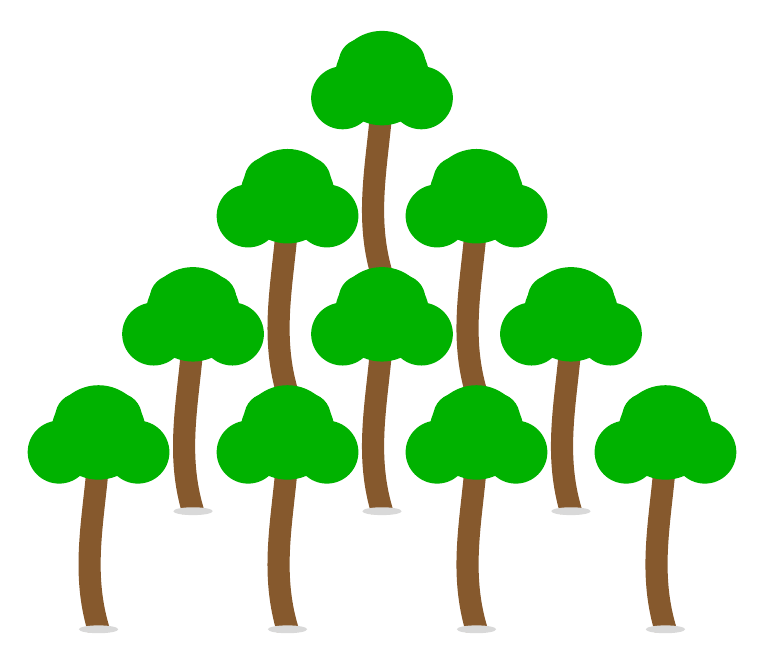
\begin{tikzpicture}
			\begin{scope}[shift={(0,0)}] \tree \end{scope}
				\foreach  \x in {-1.2,1.2}{
					\begin{scope}[shift={(\x,-1.5)}] \tree \end{scope}
				 }
				\foreach \x in {-2.4,0,2.4}{ 
					\begin{scope}[shift={(\x,-3)}] \tree \end{scope}
				} 
				\foreach \x in  {-3.6,-1.2,1.2,3.6}{
					\begin{scope}[shift={(\x,-4.5)}] \tree \end{scope}
				 }
			\end{tikzpicture}
	\end{center}
	 \choiceTF
		{\True  Số cây mỗi hàng lập thành một cấp số cộng $(u_n)$ có số hạng đầu là $u_1=1$}
		{Số cây mỗi hàng lập thành một cấp số cộng $(u_n)$ có công sai  là $d=2$}
		{\True Có tất cả $80$ hàng  cây}
		 {Hàng thứ $20$ trồng được $40$ cây}
	 \loigiai{
		\begin{itemchoice}
			\itemch Số cây mỗi hàng (bắt đầu từ hàng thứ nhất) lập thành  một cấp số cộng $(u_n)$ có $u_1=1,\, d=1$.
			\itemch  $d=1$.
			\itemch Giả sử có $n$ hàng cây thì $u_1+u_2+\cdots+u_n=3\,240={S_n}$.  \\
			 Ta có $3\,240={S_n}=n\cdot u_1+\dfrac{n\left(n-1\right)}{2}\cdot d\Leftrightarrow {n^2}+n-6\,480=0\Leftrightarrow n=80$.
			\itemch Số cây hàng thứ $20$ trồng được  là $u_{20}=u_1+19d=20$.
		\end{itemchoice}
	 }
\end{ex}

% nguồn: Ok_dungsai_lop11_Lan1
\begin{ex}%[1D2H2-3]%[ma:25cbbf6f]
 Cho cấp số cộng $\left(u_n \right)$ có số hạng đầu $u_1=\dfrac{3}{2}$, công  sai $d=\dfrac{1}{2}$. Khi đó
  \choiceTF
   {Công thức cho số hạng tổng quát $u_n=1+\dfrac{n}{3}$}
  {\True $5$ là số hạng thứ 8 của cấp số cộng đã  cho}
  {$\dfrac{15}{4}$  một số hạng của cấp số cộng đã cho}
  {Tổng $100$ số hạng đầu của cấp số cộng $\left(u_n  \right)$ bằng $2620$}
 \loigiai{ 
  \begin{itemchoice}
   \itemch Ta có $u_n=u_1+(n-1)d=\dfrac{3}{2}+(n-1)\cdot \dfrac{1}{2}=1+\dfrac{n}{2}$. 
   \itemch Xét $5=1+\dfrac{n}{2} \Rightarrow n=8\in \mathbb{N}^{*}$;  suy ra 5 là số hạng thứ 8 của cấp số cộng đã cho.
   \itemch Xét $\dfrac{15}{4}=1+\dfrac{n}{2} \Rightarrow  n=\dfrac{11}{2} \notin \mathbb{N}^{*};$ suy ra $\dfrac{15}{4}$ không là một số hạng của cấp số cộng đã cho.
   \itemch Tổng 100 số hạng đầu  của cấp số cộng là
    \[S_{100}=\dfrac{100\left[2\cdot \dfrac{3}{2}+(100-1)\cdot \dfrac{1}{2} \right]}{2}=2625.
    \]
  \end{itemchoice}
 } 
\end{ex}

% nguồn: Ok_dungsai_lop11_Lan1
\begin{ex}%[1D2H2-3]%[ma:217601f2]
 Cho cấp số  cộng $(u_n)$ có $u_4=14$, $u_6=20$. Các mệnh đề sau đúng hay sai?
 \choiceTF 
  {\True Công  sai của cấp số cộng bằng $3$}
  {Số hạng đầu  $u_1$ bằng $4$}
  {\True Số hạng thứ năm  bằng $17$}
   {Số hạng tổng quát $u_n=3n-1$}
  \loigiai{
  \begin{itemchoice}
   \itemch Ta có  $u_6-u_4=u_1+5d-u_1-3d=2d=6\Rightarrow d=3$.
   \itemch  Ta có $u_4=u_1+3d\Leftrightarrow 14=u_1+3\cdot 3\Leftrightarrow u_1=5$.
   \itemch  Ta có $u_5=u_4+d=14+3=17$.\\
   \itemch  Số hạng tổng quát $u_n=u_1+(n-1)d=5+(n-1)\cdot3=3n+2$.
  \end{itemchoice}
 } 
\end{ex}

% nguồn: Ok_dungsai_lop11_Lan1
\begin{ex}%[1D2H2-3]%[ma:dbd30c88]
 Cho cấp số cộng $\left(u_n\right)$ có  $u_3=6$ và $u_{10}=34$. Các mệnh đề sau đúng hay sai?
  \choiceTF
  {\True $\left(u_n\right)$ có  $u_1=-2$ và công sai $d=4$}
  {Tổng $10$ số hạng đầu bằng $170$} 
  {\True Số hạng thứ năm bằng $14$} 
  {Số $70$  là số hạng thứ $18$}
 \loigiai{ 
  \begin{itemchoice}
   \itemch Ta có $ \heva{&  u_1 +2d=6\\ &u_1 +9d=34 } \Rightarrow \heva{& u_1=-2 \\ &d=4.}$
   \itemch  Ta có $ S_n=nu_1+\dfrac{n(n-1)d}{2}\Rightarrow S_{10}=-2\cdot 10+\dfrac{10\cdot 9\cdot 4}{2}=172 $.
   \itemch Ta có $u_5=u_1+4d=-2+4\cdot4=14$. 
   \itemch Giả sử $70$ là số  hạng thứ $n$ của cấp số cộng.\\
    Ta có $n=\dfrac{u_n-u_1}{d}+1=\dfrac{70-(-2)}{4}+1=19$.\\
   Vậy số $70$ là số hạng thứ  $19$ của cấp số cộng $(u_n)$.
  \end{itemchoice}
 } 
\end{ex}


%%%%%%%%%%%%%%%% TRẢ LỜI NGẮN %%%%%%%%%%%%%%%%

% nguồn: Ok_TraLoiNgan_Lop11_Lan2
\begin{ex}%[1D2H2-3]%[ma:9f2c61eb]
	Cho hai số $-3$ và $23$. Xen kẽ giữa  hai số đã cho $n$ số hạng để tất cả các số đó tạo thành cấp số cộng có công sai $d=2$. Tìm $n$.
	 \shortans{12}
	\loigiai{ 
		Theo giả thiết thì ta  được một cấp số cộng có $n+2$ số hạng với $u_1=-3$; $u_{n+2}=23$.\\
		Khi đó $u_{n+2}=u_1+(n+1)\cdot d \Leftrightarrow n+1 = \dfrac{u_{n+2}-u_1}{d} = \dfrac{23-(-3)}{2} =  13 \Leftrightarrow n=12$.
	 }
\end{ex}

% nguồn: Ok_TraLoiNgan_Lop11_Lan2
\begin{ex}%[1D2H2-3]%[ma:638bb529]
	Biết các số $\mathrm{C}_{n}^{1}; \mathrm{C}_{n}^{2}; \mathrm{C}_{n}^{3}$ theo thứ tự lập thành  một cấp số cộng với $n>3$. Tìm $n$.
	\shortans{7} 
	\loigiai{ 
		Ba số $\mathrm{C}_{n}^{1}$; $\mathrm{C}_{n}^{2}$; $\mathrm{C}_{n}^{3}$ theo thứ tự $u_1$; $u_2$; $u_3$ lập thành cấp  số cộng nên
		\begin{align*}
			 &u_1+u_3=2u_2\\
			 \Leftrightarrow &\mathrm{C}_n^1+\mathrm{C}_n^3=2\mathrm{C}_n^2 \quad (n \ge 3)\\
			\Leftrightarrow &n+\dfrac{(n-2)\cdot (n-1)\cdot n}{6} = 2\cdot \dfrac{(n-1)\cdot n}{2}\\ 
			 \Leftrightarrow &\dfrac{n^2-3n+2}{6}+1 = n-1\\
			\Leftrightarrow  &n^2-9n+14=0\\
			\Leftrightarrow  &\heva{& n=2\\& n=7}\\
			\Rightarrow &n=7 \quad (n  \ge 3).
		\end{align*}
	} 
\end{ex}

% nguồn: Ok_TraLoiNgan_Lop11_Lan2
\begin{ex}%[1D2H2-3]%[ma:7c44cdb1]
	Cho cấp số cộng $(u_n)$ thoả mãn $\heva{& u_2+u_4+u_6 = 36\\& u_2\cdot u_3 = 54}$.  Tìm công sai $d$ của cấp số cộng $(u_n)$, biết $d > 4$.
	 \shortans{15}
	 \loigiai{
		Ta có 
		\begin{align*}
			&\heva{& u_2+u_4+u_6 = 36\\& u_2u_3  = 54.}\\
			\Leftrightarrow &\heva{&(u_1+d)+(u_1+3\cdot d)+(u_1+5\cdot d) = 36\\&(u_1+d)\cdot (u_1+2\cdot d) = 54}\\ 
			\Leftrightarrow &\heva{& u_1+3\cdot  d = 12 \quad (1)\\& (u_1+d)\cdot (u_1+2\cdot d) = 54. \quad (2)}
		\end{align*}
		Từ  $(1)$ suy ra $u_1 = 12-3d$ thay vào $(2)$, ta được
		$$(12-2d)\cdot (12-d) = 54 \Leftrightarrow d^2-18\cdot  d+45 = 0 \Leftrightarrow \hoac{&d=3\\&d=15.}$$
		 Vì $d > 4$ nên $d=15$ thoả mãn.
	} 
\end{ex}

% nguồn: Ok_TraLoiNgan_Lop11_Lan2
\begin{ex}%[1D2V2-3]%[ma:f53f3299]
	Ba góc $A$, $B$, $C$ $(A < B < C)$ của tam giác tạo thành cấp số cộng, biết góc lớn nhất gấp đôi góc bé  nhất. Hiệu số đo độ của góc lớn nhất với góc nhỏ nhất bằng
	\shortans{40} 
	\loigiai{ 
		Ba góc $A, B, C$ của một  tam giác theo thứ tự đó lập thành cấp số cộng thì $C+A=2B$.\\
		Ta có $\heva{&A+B+C=180^\circ\\&A+C=2B\\&C=2A} \Leftrightarrow \heva{&3B=180^\circ\\&A+C=2B\\&C=2A} \Leftrightarrow \heva{&B=60^\circ\\&A+C=120^\circ\\&C=2A} \Rightarrow \heva{&A=40^\circ\\&B=60^\circ\\&C=80^\circ} \Rightarrow C-A=40^\circ$. 
	 }
\end{ex}


%%%%%%%%%%%%%%%% TỰ LUẬN %%%%%%%%%%%%%%%%

% nguồn: Ok_TuanLuan_Toan11_Lan2
\begin{ex}%[1D2H2-3]%[ma:8f643efa]
	Cho một cấp số cộng $\left(u_{n}\right)$ có $u_{1}=5$ và tổng của $50$ số hạng  đầu bằng $5\,150$. Tìm công thức của số hạng tổng quát $u_{n}$.
	 \loigiai{Ta có $S_{50}=\dfrac{50}{2}\left(2 u_{1}+49 d\right)=5\,150 \Rightarrow d=4$.\\
	 Số hạng tổng quát của cấp số cộng là $u_{n}=u_{1}+(n-1) d=1+4 n$.}
\end{ex}

% nguồn: Ok_TuanLuan_Toan11_Lan2
\begin{ex}%[1D2H2-3]%[ma:624eaaa9]
	Cho cấp số  cộng $\left(u_{n}\right)$ có $u_{1}=3$ và công sai $d=7$. Hỏi kể từ số hạng thứ mấy trở đi thì các số hạng của $\left(u_{n}\right)$ đều lớn hơn $2\,018$?
	\loigiai{Ta có $u_{n}=u_{1}+(n-1) d=3+7(n-1)=7  n-4$.\\
		Khi đó $u_{n}>2\,018 \Leftrightarrow 7 n-4>2\,018 \Leftrightarrow n>\dfrac{2\,022}{7}\approx  288{,}9$.\\
	 Vậy kể từ số hạng thứ $289$ trở đi thì các số hạng của $\left(u_n\right)$ đều lớn hơn $2\,018$.}
\end{ex}

% nguồn: Ok_TuanLuan_Toan11_Lan2
\begin{ex}%[1D2H2-3]%[ma:c71e103f]
	 Cho cấp số cộng $\left(u_{n}\right)$ thỏa mãn $\heva{&u_4=10\\
	&u_4+u_6=26}$. Tìm công sai của cấp số cộng đã  cho.
	\loigiai{Gọi $d$ là công sai.\\ 
		Ta  có $\heva{&u_4=10\\
		&u_4+u_6=26} 
		\Leftrightarrow 
		 \heva{&u_1+3d=10\\
		 &u_1+5d=26}
		 \Leftrightarrow
		\heva{&u_1=-14\\ 
		&d=8.}$\\ 
	Vậy công  sai $d=3$.}
\end{ex}

% nguồn: Ok_TuanLuan_Toan11_Lan2
\begin{ex}%[1D2V2-3]%[ma:5c22f5e9]
	Cho cấp số cộng  $(u_n)$ có số hạng đầu ${u_1=-3}$, công sai ${d=5}$.
	\begin{enumerate}
		\item Viết  công thức của số hạng tổng quát $u_n$.
		\item Số $492$ là số hạng thứ  mấy của cấp số cộng trên?
		\item Số $300$ có là số hạng nào của cấp số cộng  trên không?
	\end{enumerate}
	\loigiai{ 
		\begin{enumerate}
			\item Ta  có $u_n=u_1+\left(n-1\right)d=-3+\left(n-1\right)5=5n-8$.
			\item Ta có ${5n-8=492\Leftrightarrow n=100}$. Vậy số $492$ là số hạng thứ  $100$ của $(u_n)$.
			\item Nhận  thấy ${5n-8=300\Leftrightarrow n=\dfrac{308}{5}=61{,}6\notin \mathbb{N}^*}$.\\ Vậy số $300$ không là số hạng nào của $(u_n)$.
		\end{enumerate}
	} 
\end{ex}

% nguồn: Ok_TuanLuan_Toan11_Lan2
\begin{ex}%[1D2V2-3]%[ma:73b46183]
	Cho cấp số cộng $(u_n)$, biết $\heva{& u_5+3u_3-u_2 = -21\\&  3u_7-2u_4 = -34.}$
	\begin{enumerate}
		\item Tìm số hạng thứ $100$  của cấp số cộng $(u_n)$.
		\item Tính tổng  của $15$ số hạng đầu tiên của cấp số cộng $(u_n)$.
		\item Tính $S = u_4+u_5+\ldots+u_{30}$. 
	\end{enumerate}
	 \loigiai{
		\begin{enumerate}
			\item Từ giả thiết của bài toán ta  có
			\begin{align*}
				&\heva{& u_1+4\cdot d+3\cdot (u_1+2\cdot d)-(u_1+d) = -21\\& 3\cdot (u_1+6\cdot d)-2(u_1+3\cdot  d) = -34}\\
				\Leftrightarrow &\heva{& u_1+3\cdot d = -7\\&  u_1+12\cdot d = -34}\\
				\Leftrightarrow &\heva{& u_1 = 2\\& d  = -3.}
			\end{align*}
			Số hạng thứ $100$ của cấp số cộng $(u_n)$ là $u_{100} = u_1+99\cdot d = 2+99\cdot (-3) =  -295$.
			\item Tổng của $15$ số hạng đầu  tiên của cấp số cộng $(u_n)$ là
			$$S_{15} = \dfrac{15\cdot (2 \cdot u_1 + 14 \cdot d)}{2}= \dfrac{15\cdot (2 \cdot 2 + 14 \cdot  (-3))}{2} = -285.$$
			 \item Ta có
			$$S= u_4+u_5+\ldots +u_{30}=  \dfrac{27\cdot (2u_4+26\cdot d)}{2}= 27\cdot (u_1+16\cdot d)= 27\cdot [2+16\cdot (-3)] = -1\,242.$$
		\end{enumerate}
	} 
\end{ex}
